\documentclass{article}
\usepackage{graphicx} % Required for inserting images
\usepackage[margin=1in]{geometry}
\usepackage{wrapfig}
\usepackage{subcaption}
\usepackage{hyperref}
\usepackage[table]{xcolor}
\newcommand{\code}[1]{\texttt{#1}}

\title{CISC856 A2: Windy Gridworld Convergence and Hyperparameters for TD Methods and Eligibility Traces}
\author{Teodor Ilie}
\date{\today}

\begin{document}

\maketitle

\textit{Note: Code is all original, with some ideas taken from \href{https://www.geeksforgeeks.org/sarsa-reinforcement-learning/}{GeeksForGeeks} for the basic Sarsa implementation.}

\section{Windy Gridworld}\label{standard_env}
First, hyperparameter choices and convergence time were compared for the regular windy gridworld environment as defined by Sutton and Barto. The environment is implemented in \code{windygridworld.WindyGridworld()}.

\subsection{Hyperparameter Choice for Sarsa, Q-Learning, Sarsa($\lambda$) and Watkins Q($\lambda$)}

\subsubsection{Hyperparameter choice for $\epsilon, \alpha$}

Hyperparameters were compared using \code{main.py}. For Sarsa, good hyperparameter options in general are $\alpha = 0.5, \epsilon = 0.1$. These are commonly used, including in the Sutton and Barto textbook on pg. 130. The same values work for Q-Learning, although other values are also commonly chosen, such as $\alpha \in [0.1, 0.5]$ and $\epsilon \in [0.1, 0.3]$. These $\alpha$ values ensure fast but stable learning, and the $\epsilon$ values are a good balance of exploration and exploitation. 

Figure \ref{fig:hyperparam} shows a graphical comparison of other value combinations. As can be seen, in this particular case, a smaller value for $\epsilon=10^{-5}$ was slightly better, and the alternatives were worse. This means a greedier action selection strategy (selecting non-optimal actions less frequently due to smaller $\epsilon$) appears to complete episodes faster while still exploring sufficiently. For the rest of the report however $\epsilon=0.1$ is used, as it works better universally, including for the stochastic King's move environment, which will be covered in section \ref{stochastic_env}.

The same parameter choices performed best for Sarsa($\lambda$) and Watkins Q($\lambda$) as well, although the graphs are not shown due to space constraints. 

\begin{figure}[h!]
  \centering
  \begin{subfigure}{0.45\textwidth} 
    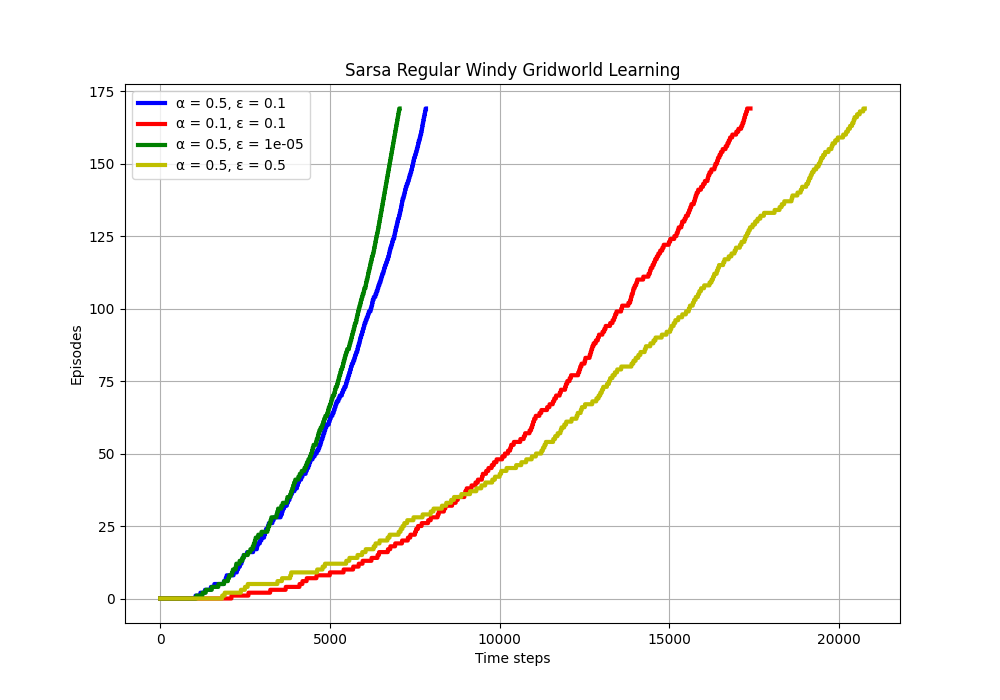
\includegraphics[width=\textwidth]{sarsa_regular.png}
    \caption{Sarsa}
  \end{subfigure}
  \hspace{0.05\textwidth}  
  \begin{subfigure}{0.45\textwidth}  
    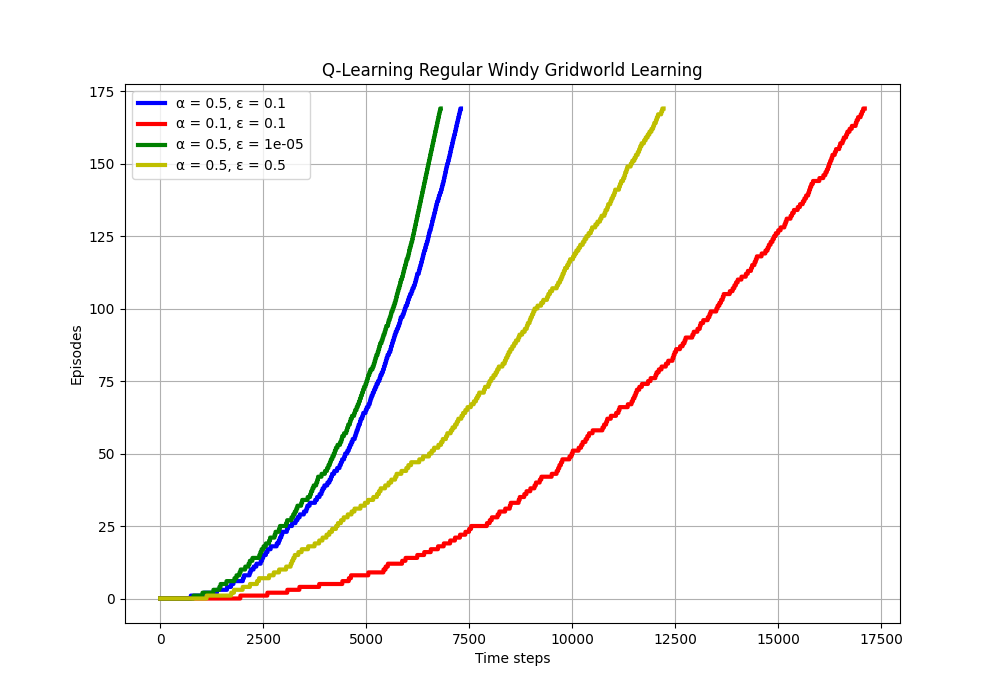
\includegraphics[width=\textwidth]{q_regular.png}
    \caption{Q-Learning}
  \end{subfigure}
  \caption{Sarsa and Q-Learning hyperparameter value comparison of $\alpha, \epsilon$ over 170 episodes, in normal windy gridworld. Values $\alpha = 0.5, \epsilon = 0.1$ performed very well, although $\alpha = 0.5, \epsilon = 10^{-5}$ performed slightly better for both methods.}
  \label{fig:hyperparam}
\end{figure}

Figure \ref{fig:regular_example} shows examples of the optimal policy learned using Sarsa and Q-Learning over 170 episodes for standard values of $\alpha = 0.5, \epsilon = 0.1$, as well as the optimal path length and average steps over the second half of all episodes. 

\begin{figure}[h!]
  \centering
  \begin{subfigure}{0.4\textwidth} 
    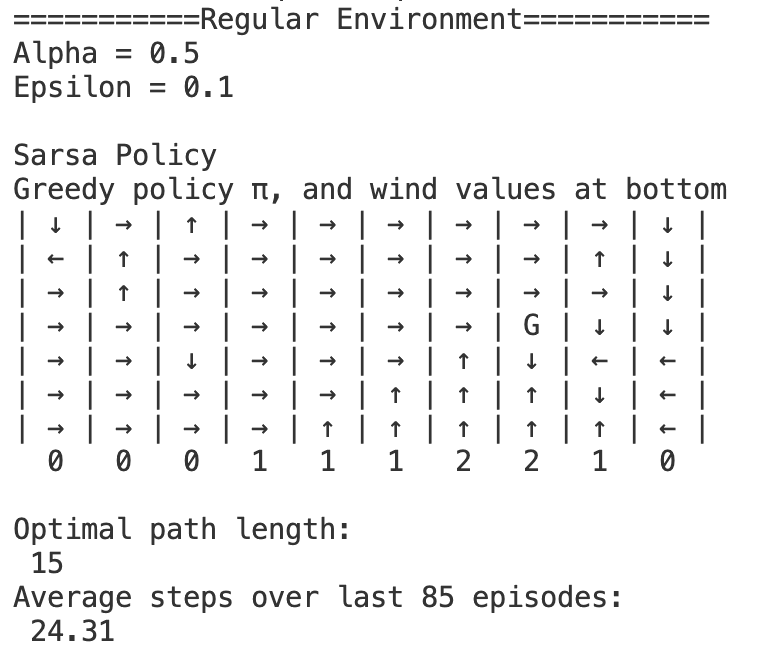
\includegraphics[width=\textwidth]{sarsa_regular_example.png}
    \caption{Sarsa}
  \end{subfigure}
  \hspace{0.05\textwidth}  
  \begin{subfigure}{0.4\textwidth}  
    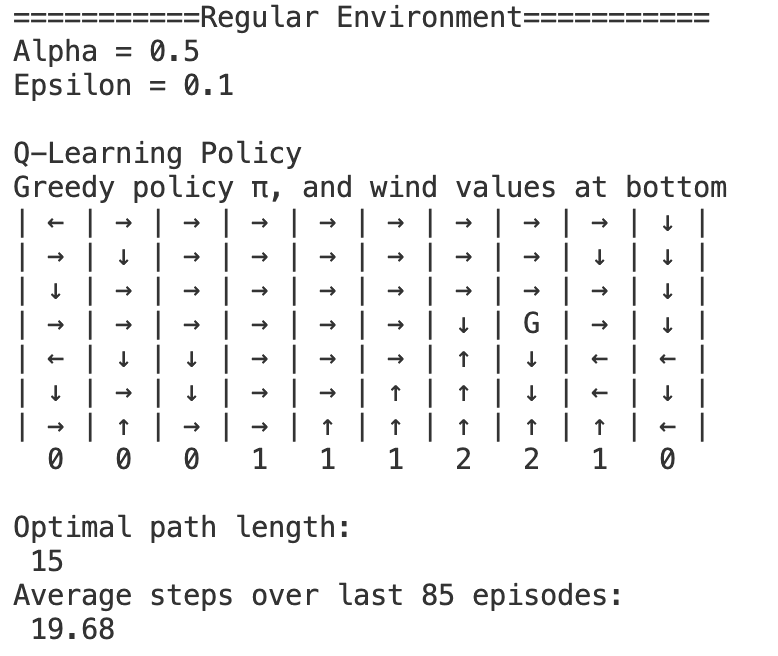
\includegraphics[width=\textwidth]{q_regular_example.png}
    \caption{Q-Learning}
  \end{subfigure}
  \caption{Sarsa and Q-Learning greedy policy and statistics, in normal windy gridworld, after 170 episodes. In these runs specifically, both methods found the optimal path with length 15. The goal state is marked $G$; the start state is at $row=4,\ col=1$, but is not marked $S$ to show the greedy action choice at that state.}
  \label{fig:regular_example}
\end{figure}

\subsubsection{Hyperparameter choice for $\lambda$ for Eligibility Trace Algorithms}

Next, Sarsa($\lambda$) and Watkins Q($\lambda$) were compared with different values for their additional hyperparameter $\lambda$, for set values of $\alpha = 0.5, \epsilon = 0.1$. The best value was found to be $\lambda=0.5$. This makes sense, as a value of $0$ corresponds to 1-step TD, and a value of $1$ corresponds to Monte Carlo, whereas a middle value like $0.5$ gives an eligibility trace that balances both, allowing the agent to learn from both immediate and past rewards.

In summary, the best hyperparameter choices were found to be $\alpha = 0.5, \epsilon = 0.1$ and $\lambda=0.5$.

\begin{figure}[h!]
  \centering
  \begin{subfigure}{0.45\textwidth} 
    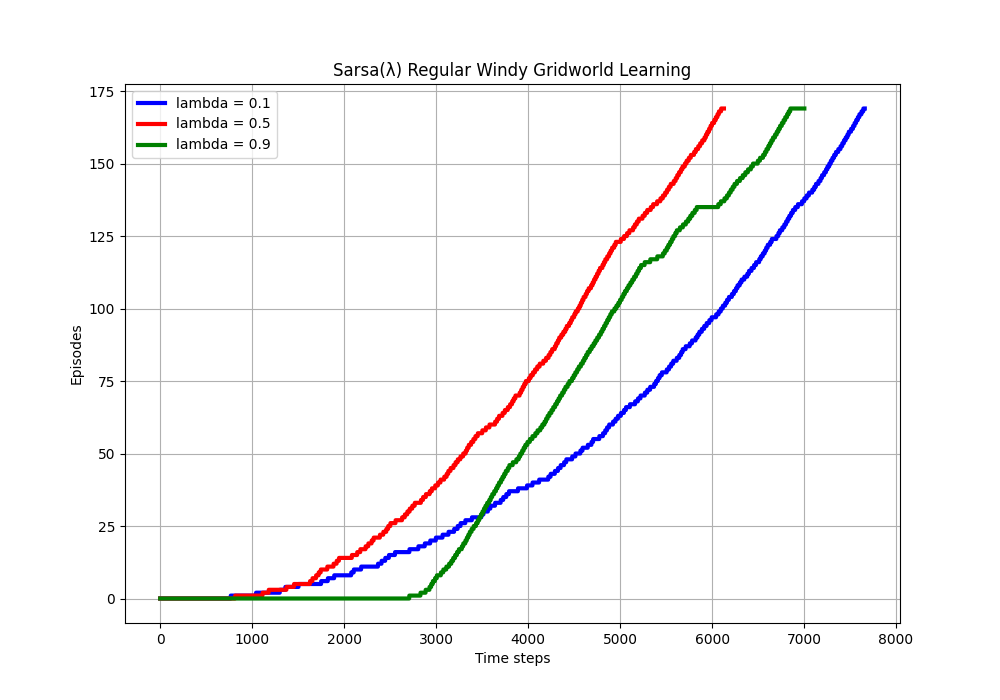
\includegraphics[width=\textwidth]{sarsa_lambda_comparison.png}
    \caption{Sarsa}
  \end{subfigure}
  \hspace{0.05\textwidth}  
  \begin{subfigure}{0.45\textwidth}  
    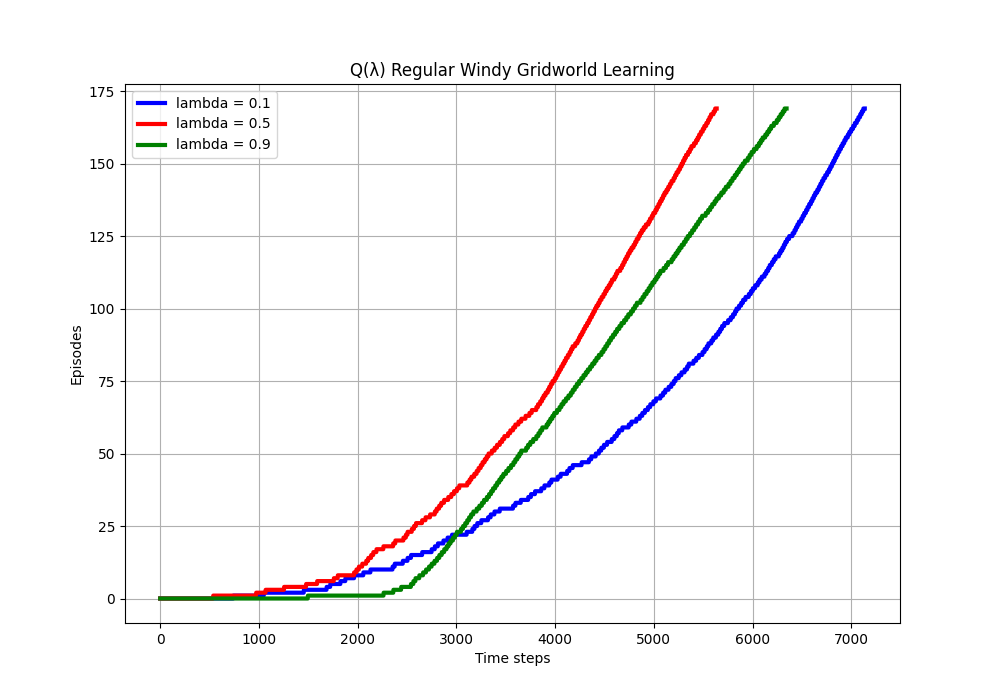
\includegraphics[width=\textwidth]{q_lambda_comparison.png}
    \caption{Q-Learning}
  \end{subfigure}
  \caption{Sarsa($\lambda$) and Watkins Q($\lambda$) comparison of hyperparameter $\lambda$ over 170 episodes, in normal gridworld. The best value was $\lambda=0.5$ for both algorithms. }
  \label{fig:lambda_comparison}
\end{figure}

\subsection{Convergence comparison for Sarsa, Q-Learning, Sarsa($\lambda$) and Watkins Q($\lambda$)} \label{convergence_regular}

Convergence was compared using \code{convergence.py}. The programs were run until the optimal path of length 15 was found; this is not the whole optimal policy, only the optimal policy for those states along the optimal path, but it is sufficient to compare convergence. To account for the stochastic nature of the algorithms, they were run until convergence 50 times, and the average performance was outputted. 

As seen in Table \ref{table:convergence}, Q-Learning outperforms Sarsa consistently for standard parameter choices. This makes sense because the off-policy nature of Q-Learning updates towards the greedy policy even when exploring, unlike on-policy Sarsa, making it faster for finding the optimal path. Additionally, both algorithms with eligibility traces outperformed their standard counterparts, as the traces allowed them to improve their learning by using past experience. 

\begin{table}[h]
    \centering
    \renewcommand{\arraystretch}{1.2}
    \begin{tabular}{|>{\columncolor{gray!30}}c|c|c|}
        \hline
        \rowcolor{gray!50}  & \textbf{Average time steps} & \textbf{Average episodes} \\
        \hline
        \textbf{Sarsa} & 6926.22 & 114.64\\
        \hline
        \textbf{Q-Learning} &  5839.4  & 95.04 \\
        \hline
        \textbf{Sarsa($\lambda$)} & 4306.88 & 87.02\\
        \hline
        \textbf{Watkins Q($\lambda$)} & 3653.56  & 66.74\\
        \hline
    \end{tabular}
    \caption{Average time steps and average episodes required to find the optimal path for different control algorithms in the regular environment. Performance from worst to best is: Sarsa, Q-Learning, Sarsa($\lambda$), and Watkins Q($\lambda$). Hyperparameter values are $\alpha = 0.5, \epsilon = 0.1$, and $\lambda=0.5$}
    \label{table:convergence}
\end{table}

\section{Stochastic Windy Gridworld}\label{stochastic_env}
Next, the modified windy grid world was investigated with stochastic wind and King's moves (the agent can move diagonally as well). It is implemented in \code{windygridworld.StochasticGridWorld()}, which inherits the regular gridworld environment and applies the changes. 

\subsection{Hyperparameter choice for Stochastic Windy Gridworld}

\subsubsection{Hyperparameter choice for $\epsilon, \alpha$}

For the stochastic King's moves gridworld environment, $\alpha = 0.5, \epsilon = 0.1$ performed the best of the hyperparameter choices, as is shown in Figure \ref{fig:stochastic_hyperparam}. The large value of $\epsilon = 0.1$ performed better than $\epsilon = 10^{-5}$, unlike regular gridworld, probably because the increased number of action options as well as the stochastic wind meant that more exploration was necessary. Learning was also less stable due to the stochastic nature of the wind, as can be seen by the graphs having a less smooth shape as compared to Figure \ref{fig:hyperparam}.

It is now shown here to save space, but in the stochastic environment, Sarsa($\lambda$) and Watkins Q($\lambda$) also performed best with the same hyperparameter choices. In addition, example policies learned are shown in Figure \ref{fig:stochastic_example_policy}. It should be noted that the shortest path, due to the ability to move diagonally, is $7$, not $15$, and that several optimal paths with the same length exist.

\begin{figure}[h!]
  \centering
  \begin{subfigure}{0.45\textwidth} 
    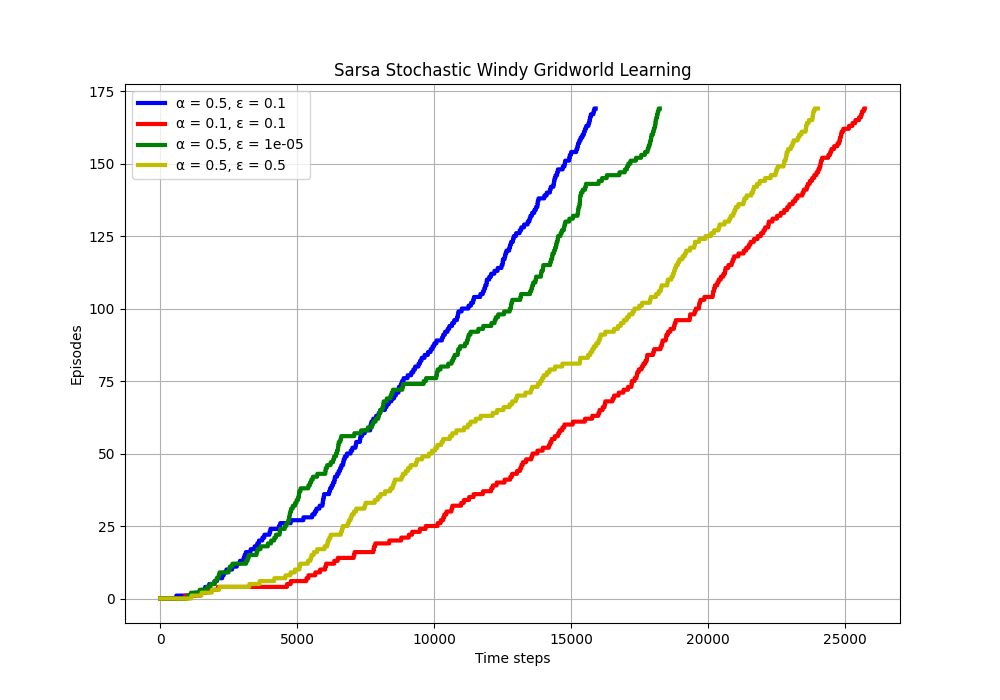
\includegraphics[width=\textwidth]{sarsa_stochastic.png}
    \caption{Sarsa}
  \end{subfigure}
  \hspace{0.05\textwidth}  
  \begin{subfigure}{0.45\textwidth}  
    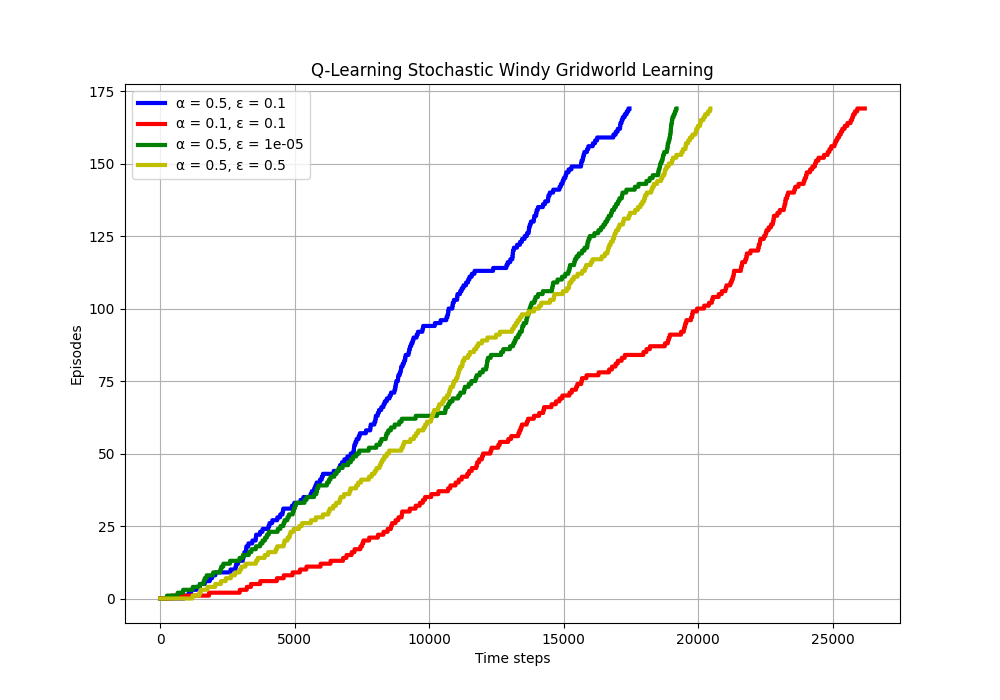
\includegraphics[width=\textwidth]{q_stochastic.png}
    \caption{Q-Learning}
  \end{subfigure}
  \caption{Sarsa and Q-Learning hyperparameter value comparison over 170 episodes, in stochastic gridworld. Standard values of $\alpha = 0.5, \epsilon = 0.1$ performed best, but learning was slower and less stable than regular gridworld due to the larger number of action choices and the stochastic environment.}
  \label{fig:stochastic_hyperparam}
\end{figure}

\begin{figure}[h!]
  \centering
  \begin{subfigure}{0.4\textwidth} 
    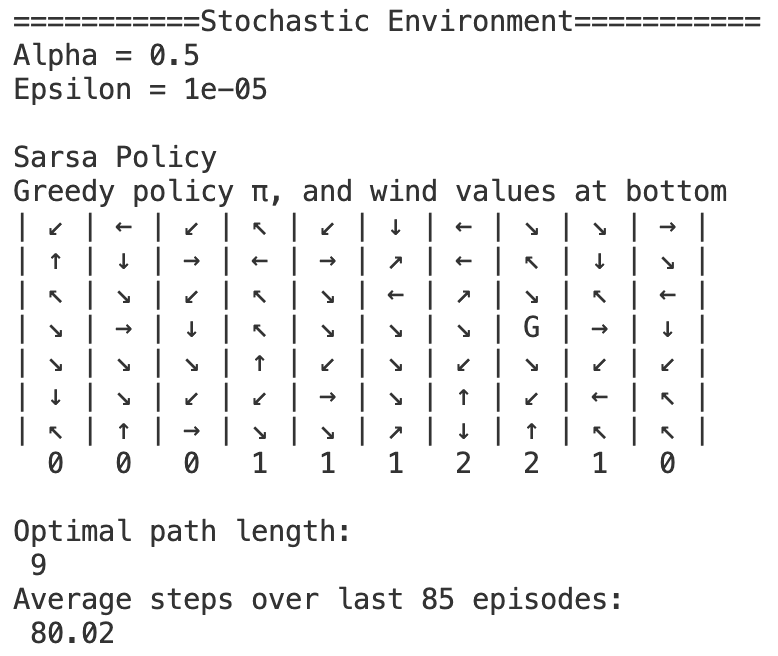
\includegraphics[width=\textwidth]{sarsa_stochastic_example.png}
    \caption{Sarsa}
  \end{subfigure}
  \hspace{0.05\textwidth}  
  \begin{subfigure}{0.4\textwidth}  
    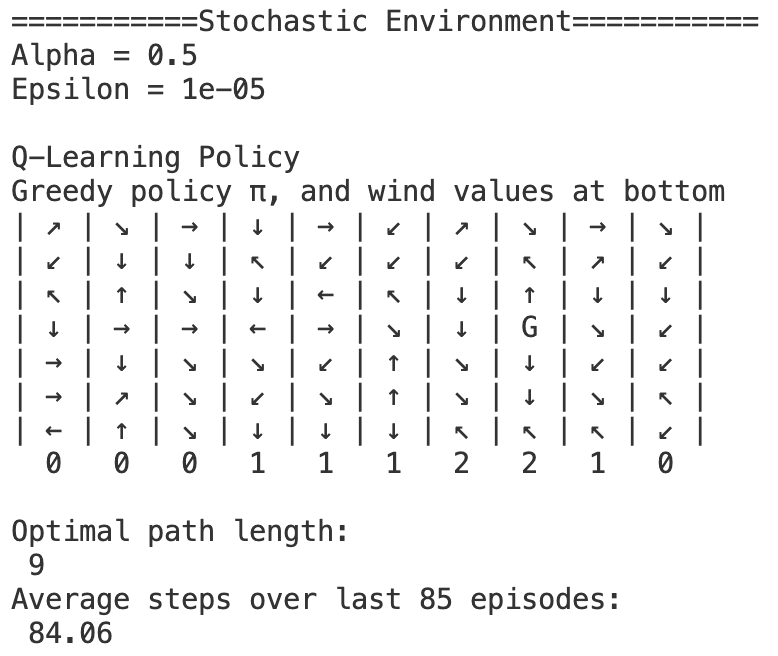
\includegraphics[width=\textwidth]{q_stochastic_example.png}
    \caption{Q-Learning}
  \end{subfigure}
  \caption{Sarsa and Q-Learning greedy policy and statistics, in stochastic gridworld, run over 1000 episodes. The optimal path length is shorter than the regular gridworld due to the diagonal movement ability.}
  
  \label{fig:stochastic_example_policy}
\end{figure}

\subsubsection{Hyperparameter choice for $\lambda$ for Eligibility Trace Algorithms}

A comparison of $\lambda$ values for the eligibility trace algorithms in the stochastic environment is shown in Figure \ref{fig:lambda_stochastic_comparison} and showed that values $0.1, 0.5$ perform similarly, but $0.9$ performs much more poorly; this is likely because the stochastic nature of the environment means less emphasis should be placed on past experience, as it can be misleading. 

\begin{figure}[h!]
  \centering
  \begin{subfigure}{0.45\textwidth} 
    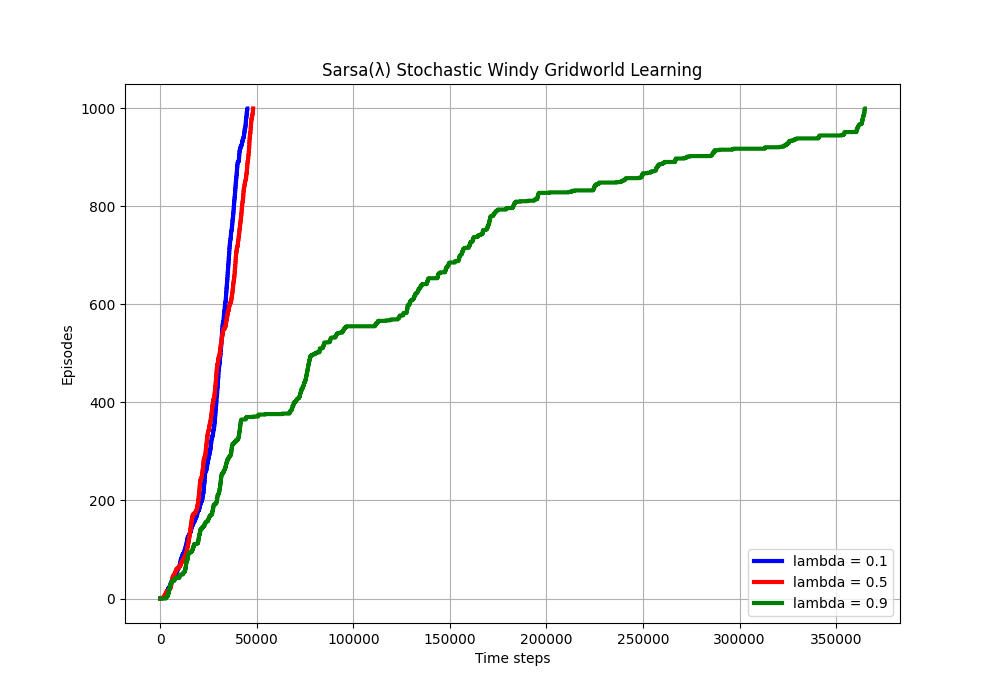
\includegraphics[width=\textwidth]{sarsa_stochastic_lambda_choice.png}
    \caption{Sarsa}
  \end{subfigure}
  \hspace{0.05\textwidth}  
  \begin{subfigure}{0.45\textwidth}  
    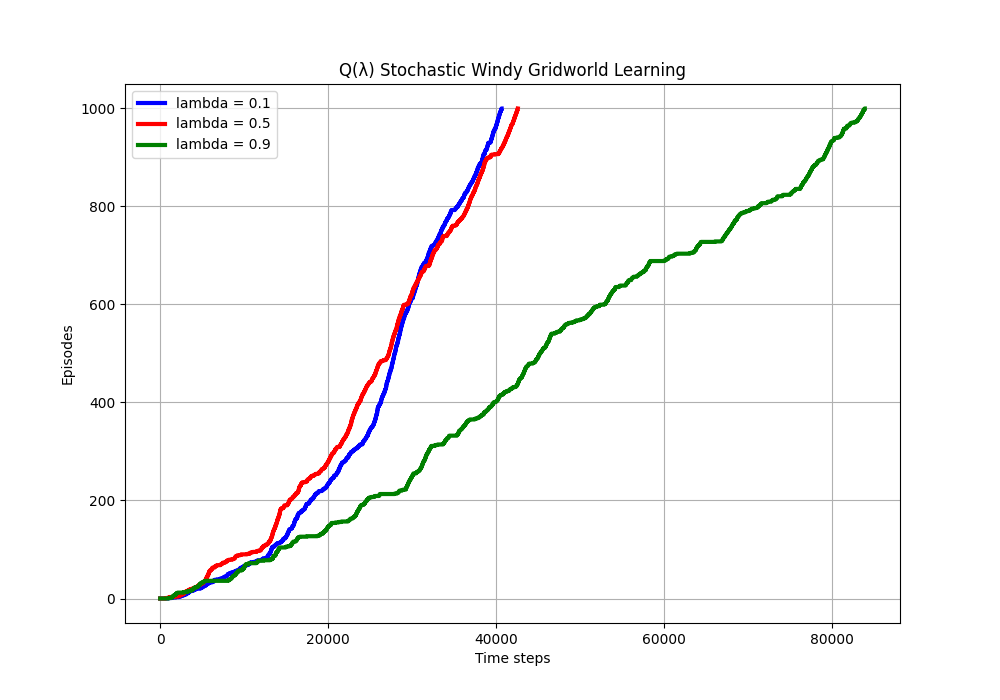
\includegraphics[width=\textwidth]{q_stochastic_lambda_choice.png}
    \caption{Q-Learning}
  \end{subfigure}
  \caption{Sarsa($\lambda$) and Watkins Q($\lambda$) comparison of hyperparameter $\lambda$ over 1000 episodes in stochastic gridworld.}
  \label{fig:lambda_stochastic_comparison}
\end{figure}

\subsection{Convergence comparison for Stochastic Windy Gridworld}

Convergence metrics were also compared in the stochastic environment, similar to Section \ref{convergence_regular}, and are shown in Table \ref{table:convergence_stochastic}. The results showed that Sarsa and Q-Learning performed similarly, while Sarsa($\lambda$) performed worse and Watkins Q($\lambda$) was worse still. This is likely because eligibility traces perform poorly in the stochastic environment. By maintaining a longer trace with noisy values, they actually perform more poorly than the 1-step lookahead used in the regular algorithms. Watkins Q(lambda) performs worse than Sarsa($\lambda$) possibly because it resets the trace when a non-greedy action is taken, whereas Sarsa maintains the information even if it is noisy.

\begin{table}[h]
    \centering
    \renewcommand{\arraystretch}{1.2}
    \begin{tabular}{|>{\columncolor{gray!30}}c|c|c|}
        \hline
        \rowcolor{gray!50}  & \textbf{Average time steps} & \textbf{Average episodes} \\
        \hline
        \textbf{Sarsa} & 13590.94 & 133.28\\
        \hline
        \textbf{Q-Learning} & 12954.78 & 133.16 \\
        \hline
        \textbf{Sarsa($\lambda$)} & 16435.04 & 211.54\\
        \hline
        \textbf{Watkins Q($\lambda$)} & 17647.0 & 267.22\\
        \hline
    \end{tabular}
    \caption{Average time steps and average episodes required to find one of the optimal paths for different control algorithms in the stochastic environment. Hyperparameter values are $\alpha = 0.5, \epsilon = 0.1, \lambda=0.5$.}
    \label{table:convergence_stochastic}
\end{table}


\end{document}
